
\begin{document}

\begin{EXO}{}{can6a-2022}


	\begin{enumerate}[itemsep=1em, label=\arabic*)]
		\item $7 \times 7=$ $\ldots$
		\item La moitié de $36$ est : \ldots
		\item Complète : \\$19+\ldots =100$ 
		\item $3$ cahiers coûtent $9$\,\euro{}.\\
				 $9$ cahiers coûtent $\ldots$\,\euro{}
		\item $2$ h $30$ min $=$
				 $\ldots$ min
		\item Quel est le nombre écrit sous le point d'interrogation ?\\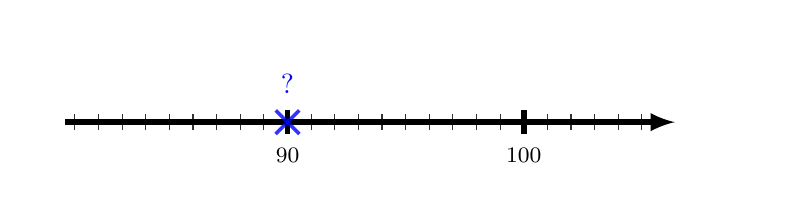
\begin{tikzpicture}[baseline,scale = 0.6]
	
		\tikzset{
		  point/.style={
			thick,
			draw,
			cross out,
			inner sep=0pt,
			minimum width=5pt,
			minimum height=5pt,
		  },
		}
		\clip (-1,-1) rectangle (15,2);
			\draw[color ={black},line width = 2,>=latex,->] (-0.2,0)--(12.7,0);
		\draw[color ={black},opacity = 0.8] (0,-0.17)--(0,0.17);
		\draw[color ={black},opacity = 0.8] (0.5,-0.17)--(0.5,0.17);
		\draw[color ={black},opacity = 0.8] (1,-0.17)--(1,0.17);
		\draw[color ={black},opacity = 0.8] (1.5,-0.17)--(1.5,0.17);
		\draw[color ={black},opacity = 0.8] (2,-0.17)--(2,0.17);
		\draw[color ={black},opacity = 0.8] (2.5,-0.17)--(2.5,0.17);
		\draw[color ={black},opacity = 0.8] (3,-0.17)--(3,0.17);
		\draw[color ={black},opacity = 0.8] (3.5,-0.17)--(3.5,0.17);
		\draw[color ={black},opacity = 0.8] (4,-0.17)--(4,0.17);
		\draw[color ={black},line width = 2] (4.5,-0.25)--(4.5,0.25);
		\draw[color ={black},opacity = 0.8] (5,-0.17)--(5,0.17);
		\draw[color ={black},opacity = 0.8] (5.5,-0.17)--(5.5,0.17);
		\draw[color ={black},opacity = 0.8] (6,-0.17)--(6,0.17);
		\draw[color ={black},opacity = 0.8] (6.5,-0.17)--(6.5,0.17);
		\draw[color ={black},opacity = 0.8] (7,-0.17)--(7,0.17);
		\draw[color ={black},opacity = 0.8] (7.5,-0.17)--(7.5,0.17);
		\draw[color ={black},opacity = 0.8] (8,-0.17)--(8,0.17);
		\draw[color ={black},opacity = 0.8] (8.5,-0.17)--(8.5,0.17);
		\draw[color ={black},opacity = 0.8] (9,-0.17)--(9,0.17);
		\draw[color ={black},line width = 2] (9.5,-0.25)--(9.5,0.25);
		\draw[color ={black},opacity = 0.8] (10,-0.17)--(10,0.17);
		\draw[color ={black},opacity = 0.8] (10.5,-0.17)--(10.5,0.17);
		\draw[color ={black},opacity = 0.8] (11,-0.17)--(11,0.17);
		\draw[color ={black},opacity = 0.8] (11.5,-0.17)--(11.5,0.17);
		\draw[color ={black},opacity = 0.8] (12,-0.17)--(12,0.17);
		\draw (4.5,-0.7) node[anchor = center] {\footnotesize \color{black}{$90$}};
		\draw (9.5,-0.7) node[anchor = center] {\footnotesize \color{black}{$100$}};
		\draw[color ={blue},line width = 1.25,opacity = 0.8] (4.25,0.25)--(4.75,-0.25);\draw[color ={blue},line width = 1.25,opacity = 0.8] (4.25,-0.25)--(4.75,0.25);
		\draw (4.5,0.8) node[anchor = center, rotate=0] {\normalsize \color{blue}{$?$}};
	
	\end{tikzpicture}
	
		\item $32+19=$$\ldots$
		\item $18$ élèves se mettent par groupe de $3$. \\
			  Il y a $\ldots$ groupes.
		\item Le tiers de $27$ est :  $\ldots$ 
		\item Complète :\\
				$4+9=\ldots+5$
		\item $4{,}4\times 10=$$\ldots$
		\item Un film commence à $19$ h $35$ et se termine à $21$ h $15$.\\
			  Combien de temps a duré le film ?
		\item Complète :\\$3=$$\ldots$ quarts
		\item Ajoute $25$ min à $7$ h $50$ min.
		\item Ajoute un dixième à $2{,}96$.
		\item Yann a $30$ billes. Il a $8$ billes de moins que Lou.\\
				   Lou a $\ldots$ billes.
		\item Le périmètre de cette figure est $26$ cm. \\
				\begin{tikzpicture}[baseline,scale = 0.8]
	
		\tikzset{
		  point/.style={
			thick,
			draw,
			cross out,
			inner sep=0pt,
			minimum width=5pt,
			minimum height=5pt,
		  },
		}
		\clip (-1.5,-1) rectangle (5,4);
			\draw [color={black}] (2,-0.5) node[anchor = center,scale=1, rotate = 0] {8,5 cm};
		\draw [color={black}] (2,3.5) node[anchor = center,scale=1, rotate = 0] {8,5 cm};
		\draw [color={black}] (4.5,1.5) node[anchor = center,scale=1, rotate = 0] {?};
		\draw[color ={black}] (0,0)--(4,0);
		\draw[color ={black}] (4,0)--(4,3);
		\draw[color ={black}] (4,3)--(0,3);
		\draw[color ={black}] (0,3)--(0,0);
		\draw[color={black},line width = 0.5] (4,0)--(3.6,0)--(3.6,0.4)--(4,0.4)--cycle;
		\draw[color={black},line width = 0.5] (4,3)--(4,2.6)--(3.6,2.6)--(3.6,3)--cycle;
		\draw[color={black},line width = 0.5] (0,3)--(0.4,3)--(0.4,2.6)--(0,2.6)--cycle;
		\draw[color={black},line width = 0.5] (0,0)--(0,0.4)--(0.4,0.4)--(0.4,0)--cycle;
	
	\end{tikzpicture}
	  $\text{?}=\ldots$ cm
		\item $0{,}2$ kg  $=$   $\ldots$ g
		\item Écris en chiffres : \\
				  Deux-millions-deux-mille 
		\item Quelle est la longueur du segment $[AB]$ ? \\
				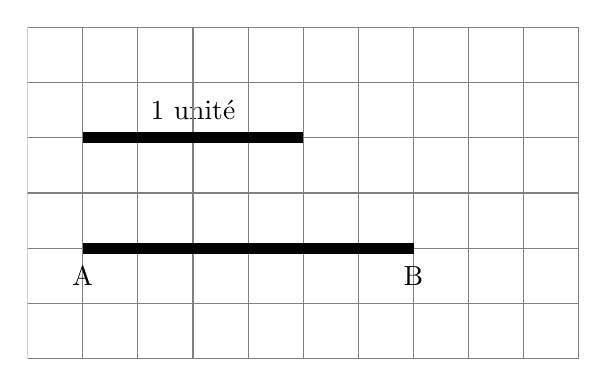
\begin{tikzpicture}[baseline,scale = 0.7]
	
		\tikzset{
		  point/.style={
			thick,
			draw,
			cross out,
			inner sep=0pt,
			minimum width=5pt,
			minimum height=5pt,
		  },
		}
		\clip (-1,-2) rectangle (9,4);
			\draw [color={black}] (2,2.5) node[anchor = center,scale=1, rotate = 0] {1 unité};
		\draw[color ={gray}] (-2,-2)--(-2,4);
		\draw[color ={gray}] (-1,-2)--(-1,4);
		\draw[color ={gray}] (0,-2)--(0,4);
		\draw[color ={gray}] (1,-2)--(1,4);
		\draw[color ={gray}] (2,-2)--(2,4);
		\draw[color ={gray}] (3,-2)--(3,4);
		\draw[color ={gray}] (4,-2)--(4,4);
		\draw[color ={gray}] (5,-2)--(5,4);
		\draw[color ={gray}] (6,-2)--(6,4);
		\draw[color ={gray}] (7,-2)--(7,4);
		\draw[color ={gray}] (8,-2)--(8,4);
		\draw[color ={gray}] (9,-2)--(9,4);
		\draw[color ={gray}] (-2,-2)--(9,-2);
		\draw[color ={gray}] (-2,-1)--(9,-1);
		\draw[color ={gray}] (-2,0)--(9,0);
		\draw[color ={gray}] (-2,1)--(9,1);
		\draw[color ={gray}] (-2,2)--(9,2);
		\draw[color ={gray}] (-2,3)--(9,3);
		\draw[color ={gray}] (-2,4)--(9,4);
		\draw[color ={black},line width = 4] (0,2)--(4,2);
		\draw[color ={black},line width = 4] (0,0)--(6,0);
		\draw [color={black}] (0,-0.5) node[anchor = center,scale=1, rotate = 0] {A};
		\draw [color={black}] (6,-0.5) node[anchor = center,scale=1, rotate = 0] {B};
	
	\end{tikzpicture}
	 \\$\ldots$ unité
		\item Complète : \\
				$10$ jours $=$$\ldots$ h
		\item Complète : \\
			  $9$ heures $=$$\ldots$ min
		\item Combien faut-il de pièces de $10$ centimes pour avoir $5{,}80$\,\euro{}. \\
						
		\item Détermine l'abscisse du point A  :\\ On donnera le résultat sous  forme décimale.\\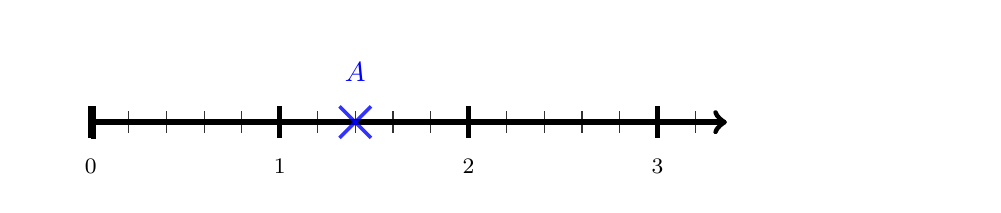
\begin{tikzpicture}[baseline,scale = 0.8]
	
		\tikzset{
		  point/.style={
			thick,
			draw,
			cross out,
			inner sep=0pt,
			minimum width=5pt,
			minimum height=5pt,
		  },
		}
		\clip (-1,-1) rectangle (14,1.5);
			\draw[color ={black},line width = 2,|->] (0,0)--(10.1,0);
		\draw[color ={black},line width = 2] (0,-0.25)--(0,0.25);
		\draw[color ={black},opacity = 0.8] (0.6,-0.17)--(0.6,0.17);
		\draw[color ={black},opacity = 0.8] (1.2,-0.17)--(1.2,0.17);
		\draw[color ={black},opacity = 0.8] (1.8,-0.17)--(1.8,0.17);
		\draw[color ={black},opacity = 0.8] (2.4,-0.17)--(2.4,0.17);
		\draw[color ={black},line width = 2] (3,-0.25)--(3,0.25);
		\draw[color ={black},opacity = 0.8] (3.6,-0.17)--(3.6,0.17);
		\draw[color ={black},opacity = 0.8] (4.2,-0.17)--(4.2,0.17);
		\draw[color ={black},opacity = 0.8] (4.8,-0.17)--(4.8,0.17);
		\draw[color ={black},opacity = 0.8] (5.4,-0.17)--(5.4,0.17);
		\draw[color ={black},line width = 2] (6,-0.25)--(6,0.25);
		\draw[color ={black},opacity = 0.8] (6.6,-0.17)--(6.6,0.17);
		\draw[color ={black},opacity = 0.8] (7.2,-0.17)--(7.2,0.17);
		\draw[color ={black},opacity = 0.8] (7.8,-0.17)--(7.8,0.17);
		\draw[color ={black},opacity = 0.8] (8.4,-0.17)--(8.4,0.17);
		\draw[color ={black},line width = 2] (9,-0.25)--(9,0.25);
		\draw[color ={black},opacity = 0.8] (9.6,-0.17)--(9.6,0.17);
		\draw (0,-0.7) node[anchor = center] {\footnotesize \color{black}{$0$}};
		\draw (3,-0.7) node[anchor = center] {\footnotesize \color{black}{$1$}};
		\draw (6,-0.7) node[anchor = center] {\footnotesize \color{black}{$2$}};
		\draw (9,-0.7) node[anchor = center] {\footnotesize \color{black}{$3$}};
		\draw[color ={blue},line width = 1.25,opacity = 0.8] (3.95,0.25)--(4.45,-0.25);\draw[color ={blue},line width = 1.25,opacity = 0.8] (3.95,-0.25)--(4.45,0.25);
		\draw (4.199999999999999,0.8) node[anchor = center, rotate=0] {\normalsize \color{blue}{$A$}};
	
	\end{tikzpicture}
	
		\item $0{,}33+0{,}4=$$\ldots$ 
		\item Choisis parmi les propositions suivantes la taille d'une girafe (nombre et unité à recopier).\\$42$ m \,\,\,\, $42$ mm \,\,\,\, $42$ cm\,\,\,\, $42$ dm
		\item Le double de $4{,}8$ est $\ldots$
		\item Compléter :\\ $ .... \times 6=36$
		\item $10$ cubes identiques empilés ont une hauteur de $50$ cm.\\
			  $15$ cubes empilés ont une hauteur de $\ldots$ cm
		\item Un bus met $2$ heures pour emmener $9$ passagers.\\
			  Combien d'heures, ce même bus mettra-t-il pour emmener $18$ passagers ?
	\end{enumerate}
	\end{EXO}
	

	
% @see : https://coopmaths.fr/alea?uuid=57239&id=canc3a-2023&n=30&d=10&alea=GnrL&cd=1&cols=1
\begin{EXO}{}{canc3a-2023}


\begin{enumerate}[itemsep=1em, label=\arabic*)]
	\item $9 \times 4$
	\item $36+29$
	\item Combien y a-t-il de boules noires ? \\ 

\begin{tikzpicture}[baseline,scale = 0.3]

    \tikzset{
      point/.style={
        thick,
        draw,
        cross out,
        inner sep=0pt,
        minimum width=5pt,
        minimum height=5pt,
      },
    }
    \clip (-0.7,-2.7) rectangle (7.7,0.7);
    	
	 \filldraw[color={black},fill={black}] (0,0) circle (0.2);
	
	 \filldraw[color={black},fill={black}] (1,0) circle (0.2);
	
	 \filldraw[color={black},fill={black}] (2,0) circle (0.2);
	
	 \filldraw[color={black},fill={black}] (3,0) circle (0.2);
	
	 \filldraw[color={black},fill={black}] (4,0) circle (0.2);
	
	 \filldraw[color={black},fill={black}] (5,0) circle (0.2);
	
	 \filldraw[color={black},fill={black}] (6,0) circle (0.2);
	
	 \filldraw[color={black},fill={black}] (7,0) circle (0.2);
	
	 \filldraw[color={black},fill={black}] (0,-1) circle (0.2);
	
	 \filldraw[color={black},fill={black}] (1,-1) circle (0.2);
	
	 \filldraw[color={black},fill={black}] (2,-1) circle (0.2);
	
	 \filldraw[color={black},fill={black}] (3,-1) circle (0.2);
	
	 \filldraw[color={black},fill={black}] (4,-1) circle (0.2);
	
	 \filldraw[color={black},fill={black}] (5,-1) circle (0.2);
	
	 \filldraw[color={black},fill={black}] (6,-1) circle (0.2);
	
	 \filldraw[color={black},fill={black}] (7,-1) circle (0.2);
	
	 \filldraw[color={black},fill={black}] (0,-2) circle (0.2);
	
	 \filldraw[color={black},fill={black}] (1,-2) circle (0.2);
	
	 \filldraw[color={black},fill={black}] (2,-2) circle (0.2);
	
	 \filldraw[color={black},fill={black}] (3,-2) circle (0.2);
	
	 \filldraw[color={black},fill={black}] (4,-2) circle (0.2);
	
	 \filldraw[color={black},fill={black}] (5,-2) circle (0.2);
	
	 \filldraw[color={black},fill={black}] (6,-2) circle (0.2);
	
	 \filldraw[color={black},fill={black}] (7,-2) circle (0.2);

\end{tikzpicture}

	\item La moitié de $42$
	\item Complète \\ {\Reperage[ValeurOrigine=70,ValeurUnitex=80,Pasx=2,AffichageAbs=3,AffichageGrad]{1/A}}
	\item Complète :  $\ldots \times \ldots =35$
	\item \Temps{;;;;35;}+ \Temps{;;;;40;}
	\item Pour partager $30$ oeufs, combien de boites de  $6$ oeufs dois-je utiliser ? 
	\item Choisis parmi les propositions suivantes la hauteur d'une bouteille.\\\Lg[dm]{33} \,\,\,\, \Lg[cm]{33} \,\,\,\, \Lg[mm]{33}\,\,\,\, \Lg[m]{33}
	\item Écris en chiffres le nombre cinquante-deux-mille-sept.
	\item Karole a $12$ ans. \\
        Laurent a 5 ans de moins que Karole. Laurent a $\ldots$ ans
	\item Donne l'écriture décimale de  $3\times 7$ centièmes.
	\item Complète \\ {\Reperage[DemiDroite,Pasx=1,Unitex=0.4,ValeurUnitex=4,AffichageAbs=2]{9/3*A,10/B}}
	\item Complète : \,\,\,
    $1{,}8+\ldots =10$ 
	\item Complète : \,\,\,
    $405= \ldots$ dizaines  $\ldots$  unités
	\item Quelle fraction de la surface totale représente la surface grisée ?
    \\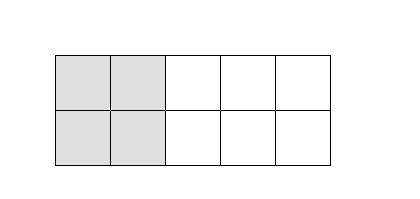
\begin{tikzpicture}[baseline,scale = 0.7]

    \tikzset{
      point/.style={
        thick,
        draw,
        cross out,
        inner sep=0pt,
        minimum width=5pt,
        minimum height=5pt,
      },
    }
    \clip (-0.5,-0.1) rectangle (6.1,2.5);
    	\draw[color={black},preaction={fill,color = {lightgray}, opacity = 0.5}] (0,0)--(2,0)--(2,2)--(0,2)--(0,2)--(0,2)--cycle;
	\draw[color ={black}] (0,0)--(0,2);
	\draw[color ={black}] (1,0)--(1,2);
	\draw[color ={black}] (2,0)--(2,2);
	\draw[color ={black}] (3,0)--(3,2);
	\draw[color ={black}] (4,0)--(4,2);
	\draw[color ={black}] (5,0)--(5,2);
	\draw[color ={black}] (0,0)--(5,0);
	\draw[color ={black}] (0,1)--(5,1);
	\draw[color ={black}] (0,2)--(5,2);

\end{tikzpicture}

	\item $25\div 5$
	\item Si $2$ cahiers coûtent $8$\,\euro{}, alors $8$ cahiers coûtent  $\ldots$\,\euro{}.
	\item Quelle est la longueur de la ligne en pointillé ? \\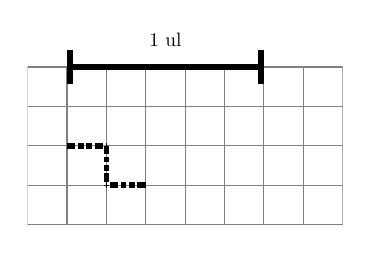
\begin{tikzpicture}[baseline,scale = 0.5]

    \tikzset{
      point/.style={
        thick,
        draw,
        cross out,
        inner sep=0pt,
        minimum width=5pt,
        minimum height=5pt,
      },
    }
    \clip (-1,-0.2) rectangle (7,5);
    	\draw [color={black}] (2.5,4.7) node[anchor = center,scale=0.7, rotate = 0] {1 ul};
	\draw[color ={gray}] (-2,0)--(-2,4);
	\draw[color ={gray}] (-1,0)--(-1,4);
	\draw[color ={gray}] (0,0)--(0,4);
	\draw[color ={gray}] (1,0)--(1,4);
	\draw[color ={gray}] (2,0)--(2,4);
	\draw[color ={gray}] (3,0)--(3,4);
	\draw[color ={gray}] (4,0)--(4,4);
	\draw[color ={gray}] (5,0)--(5,4);
	\draw[color ={gray}] (6,0)--(6,4);
	\draw[color ={gray}] (7,0)--(7,4);
	\draw[color ={gray}] (-2,0)--(7,0);
	\draw[color ={gray}] (-2,1)--(7,1);
	\draw[color ={gray}] (-2,2)--(7,2);
	\draw[color ={gray}] (-2,3)--(7,3);
	\draw[color ={gray}] (-2,4)--(7,4);
	\draw[color ={black},line width = 2,|-|] (0,4)--(5,4);
	\draw[color ={black},line width = 2, densely dash dot dot ] (0,2)--(1,2);
	\draw[color ={black},line width = 2, densely dash dot dot ] (1,2)--(1,1);
	\draw[color ={black},line width = 2, densely dash dot dot ] (2,1)--(1,1);

\end{tikzpicture}
\\
	\item  $92\times 5$
	\item Une voiture roule à $80$ km/h à vitesse constante. \\Combien de kilomètres parcourt-elle en $15$ min à cette vitesse ?
	\item Une voiture roule à  $80$ km/h à vitesse constante.\\ Combien de kilomètres parcourt-elle en $1$ h et $15$ min à cette vitesse ?
	\item Dans $32$ combien de fois $4$ ?
	\item Complète : \,\,\,
    $7$ centaines et  $\ldots$  dizaines font  $740$.
	\item Magalie veut construire une figure d'aire 6 unités d'aire (uA).\\
    
      Combien de petits carreaux doit-elle contenir ?\\    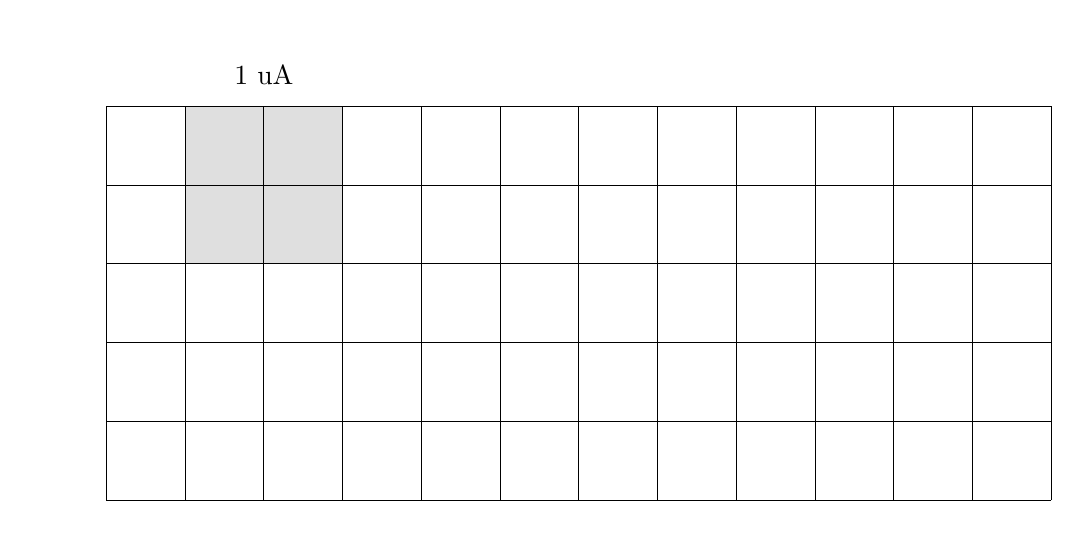
\begin{tikzpicture}[baseline]

    \tikzset{
      point/.style={
        thick,
        draw,
        cross out,
        inner sep=0pt,
        minimum width=5pt,
        minimum height=5pt,
      },
    }
    \clip (-1,-0.1) rectangle (12.1,6);
    	\draw[color={black},preaction={fill,color = {lightgray}, opacity = 0.5}] (1,5)--(3,5)--(3,3)--(1,3)--cycle;
	\draw[color ={black}] (0,0)--(0,5);
	\draw[color ={black}] (1,0)--(1,5);
	\draw[color ={black}] (2,0)--(2,5);
	\draw[color ={black}] (3,0)--(3,5);
	\draw[color ={black}] (4,0)--(4,5);
	\draw[color ={black}] (5,0)--(5,5);
	\draw[color ={black}] (6,0)--(6,5);
	\draw[color ={black}] (7,0)--(7,5);
	\draw[color ={black}] (8,0)--(8,5);
	\draw[color ={black}] (9,0)--(9,5);
	\draw[color ={black}] (10,0)--(10,5);
	\draw[color ={black}] (11,0)--(11,5);
	\draw[color ={black}] (12,0)--(12,5);
	\draw[color ={black}] (0,0)--(12,0);
	\draw[color ={black}] (0,1)--(12,1);
	\draw[color ={black}] (0,2)--(12,2);
	\draw[color ={black}] (0,3)--(12,3);
	\draw[color ={black}] (0,4)--(12,4);
	\draw[color ={black}] (0,5)--(12,5);
	\draw [color={black}] (2,5.4) node[anchor = center,scale=1, rotate = 0] {1 uA};

\end{tikzpicture}

	\item Combien de dixièmes y a-t-il en tout dans $8{,}48$ ?
	\item $6$ cahiers coûtent  $1{,}20$\,\euro{}. \\
Combien coûtent $2$ cahiers ?
	\item Le rectangle B est une réduction du rectangle A.\\ Quelle est la largeur du rectangle B ?\\\begin{tikzpicture}[baseline,scale = 0.7]

    \tikzset{
      point/.style={
        thick,
        draw,
        cross out,
        inner sep=0pt,
        minimum width=5pt,
        minimum height=5pt,
      },
    }
    \clip (-1,-0.5) rectangle (8.5,2.5);
    	\draw[color={black}] (0,0)--(2.5,0)--(2.5,1)--(0,1)--cycle;
	\draw[color={black}] (3,0)--(7,0)--(7,2)--(3,2)--cycle;
	\draw [color={black}] (7.7,1) node[anchor = center,scale=0.7, rotate = 0] {5 cm};
	\draw [color={black}] (5,-0.3) node[anchor = center,scale=0.7, rotate = 0] {8 cm};
	\draw [color={black}] (1.25,-0.3) node[anchor = center,scale=0.7, rotate = 0] {4 cm};
	\draw [color={black}] (5,1) node[anchor = center,scale=0.7, rotate = 0] {A };
	\draw [color={black}] (1.25,0.5) node[anchor = center,scale=0.7, rotate = 0] {B };

\end{tikzpicture}

	\item $1{,}93+ 0{,}8$
	\item À la cantine, il y a toujours $3$ entrées différentes, $2$ plats différents et $2$ desserts différents.\\
Combien de menus (composés d'une entrée, d'un plat et d'un dessert) différents peut-on avoir dans cette cantine ?
\end{enumerate}
\end{EXO}

% @see : https://coopmaths.fr/alea?uuid=32a0f&id=canc3a&n=30&d=10&alea=oBVG&cd=1&cols=2
\begin{EXO}{}{canc3a}

\begin{multicols}{2}
\begin{enumerate}[itemsep=1em, label=\arabic*)]
	\item \begin{minipage}[t]{\linewidth} $22+13$ \end{minipage}
	\item \begin{minipage}[t]{\linewidth} $65-32$ \end{minipage}
	\item \begin{minipage}[t]{\linewidth} $17+25$ \end{minipage}
	\item \begin{minipage}[t]{\linewidth} $83-25$ \end{minipage}
	\item \begin{minipage}[t]{\linewidth} $3\times 1\,000 + 6\times 10 + 5\times 100$ \end{minipage}
	\item \begin{minipage}[t]{\linewidth} $40\div5$ \end{minipage}
	\item \begin{minipage}[t]{\linewidth} $2{,}2+3$ \end{minipage}
	\item \begin{minipage}[t]{\linewidth} $1{,}4+1{,}16$ \end{minipage}
	\item \begin{minipage}[t]{\linewidth} $5{,}63-2{,}2$ \end{minipage}
	\item \begin{minipage}[t]{\linewidth} $6{,}1-4{,}5$ \end{minipage}
	\item \begin{minipage}[t]{\linewidth} J'ai $18$ ans. Je suis $2$ fois plus âgé que Joachim.\\Quel âge a Joachim ? \end{minipage}
	\item \begin{minipage}[t]{\linewidth} Aude participe à une course par étapes. La première étape fait $18$ km, la deuxième fait $12$ km et la dernière fait $29$ km.\\Combien de kilomètres Aude a-t-elle parcourus ? \end{minipage}
	\item \begin{minipage}[t]{\linewidth} Léa a $17$ ans. Sa sœur a $5$ ans.\\Quelle est leur différence d'âge ? \end{minipage}
	\item \begin{minipage}[t]{\linewidth} Joachim a couru $2$ séquences de $10$ minutes. Combien de minutes a-t-il couru en tout ? \end{minipage}
	\item \begin{minipage}[t]{\linewidth} Les fraises sont vendus $7{,}50$\,\euro{}~par kilogramme. Fernando en achète $3$ kg. Combien va-t-il payer ? \end{minipage}
	\item \begin{minipage}[t]{\linewidth} $\ldots - 3=2{,}2$ \end{minipage}
	\item \begin{minipage}[t]{\linewidth} $5 \times 6$ \end{minipage}
	\item \begin{minipage}[t]{\linewidth} $6 \times 4$ \end{minipage}
	\item \begin{minipage}[t]{\linewidth} On a coupé $4{,}1$ cm d'une ficelle qui en faisait $7{,}2$.\\Combien de centimètres en reste-t-il ? \end{minipage}
	\item \begin{minipage}[t]{\linewidth} \begin{tikzpicture}[baseline]

    \tikzset{
      point/.style={
        thick,
        draw,
        cross out,
        inner sep=0pt,
        minimum width=5pt,
        minimum height=5pt,
      },
    }
    \clip (-0.1,-1.5) rectangle (5.1,1.5);
    	\draw[color ={black},|-|] (0,0)--(5,0);
	\draw[color ={red},<->] (0,0.5)--(5,0.5);
	\draw [color={black}] (2.5,1) node[anchor = center,scale=1, rotate = 0] {?};
	\draw[color ={black},|-|] (0,0)--(2.97,0);
	\draw[color ={blue},<->] (0,-1)--(2.97,-1);
	\draw [color={black}] (1.49,-0.5) node[anchor = center,scale=1, rotate = 0] {3,5};
	\draw[color ={green},<->] (2.97,-1)--(5,-1);
	\draw [color={black}] (3.99,-0.5) node[anchor = center,scale=1, rotate = 0] {2,4};

\end{tikzpicture}
 \end{minipage}
	\item \begin{minipage}[t]{\linewidth} $8 \times 7$ \end{minipage}
	\item \begin{minipage}[t]{\linewidth} Quel est le périmètre de ce polygone ?\\\begin{tikzpicture}[baseline,scale = 0.8]

    \tikzset{
      point/.style={
        thick,
        draw,
        cross out,
        inner sep=0pt,
        minimum width=5pt,
        minimum height=5pt,
      },
    }
    \clip (-2.5,-1) rectangle (3,5);
    	\draw[color={black}] (-2,0)--(2,0)--(0,3.46)--cycle;
	\draw [color={black}] (0,-0.5) node[anchor = center,scale=1, rotate = 0] {5,3 cm};
	\draw [color={red}] (0,0) node[anchor = center,scale=1, rotate = 0] {//};
\draw [color={red}] (1,1.73) node[anchor = center,scale=1, rotate = -60] {//};
\draw [color={red}] (-1,1.73) node[anchor = center,scale=0.5, rotate = -300] {//};


\end{tikzpicture}
 \end{minipage}
	\item \begin{minipage}[t]{\linewidth} $\ldots \times 20=190$ \end{minipage}
	\item \begin{minipage}[t]{\linewidth} $3$ kg de fraises coûtent $22{,}5$\,\euro{}, combien coûtent $12$ kg de fraises ? \end{minipage}
	\item \begin{minipage}[t]{\linewidth} $\ldots \times 4=40$ \end{minipage}
	\item \begin{minipage}[t]{\linewidth} Le diamètre d'un cercle de $60$ unités de rayon. \end{minipage}
	\item \begin{minipage}[t]{\linewidth} \begin{tikzpicture}[baseline]

    \tikzset{
      point/.style={
        thick,
        draw,
        cross out,
        inner sep=0pt,
        minimum width=5pt,
        minimum height=5pt,
      },
    }
    \clip (-0.1,-1.5) rectangle (5.1,1.5);
    	\draw[color ={black},|-|] (0,0)--(5,0);
	\draw[color ={green},<->] (0,0.5)--(5,0.5);
	\draw [color={black}] (2.5,1) node[anchor = center,scale=1, rotate = 0] {71};
	\draw[color ={black},|-|] (0,0)--(1.97,0);
	\draw[color ={blue},<->] (0,-1)--(1.97,-1);
	\draw [color={black}] (0.99,-0.5) node[anchor = center,scale=1, rotate = 0] {28};
	\draw[color ={red},<->] (1.97,-1)--(5,-1);
	\draw [color={black}] (3.49,-0.5) node[anchor = center,scale=1, rotate = 0] {?};

\end{tikzpicture}
 \end{minipage}
	\item \begin{minipage}[t]{\linewidth} Le film a commencé à $20$ h $30$. Il s'est terminé à $22$ h $25$.\\ Combien de minutes a-t-il duré ? \end{minipage}
	\item \begin{minipage}[t]{\linewidth} En $24$ minutes, un manège fait $27$ tours.\\En $8$ minutes il fait \ldots tours. \end{minipage}
	\item \begin{minipage}[t]{\linewidth} \begin{tikzpicture}[baseline]

    \tikzset{
      point/.style={
        thick,
        draw,
        cross out,
        inner sep=0pt,
        minimum width=5pt,
        minimum height=5pt,
      },
    }
    \clip (-0.1,-1.5) rectangle (5.1,1.5);
    	\draw[color ={black},|-|] (0,0)--(5,0);
	\draw[color ={red},<->] (0,0.5)--(5,0.5);
	\draw [color={black}] (2.5,1) node[anchor = center,scale=1, rotate = 0] {?};
	\draw[color ={black},|-|] (0,0)--(1.8,0);
	\draw[color ={blue},<->] (0,-1)--(1.8,-1);
	\draw [color={black}] (0.9,-0.5) node[anchor = center,scale=1, rotate = 0] {22};
	\draw[color ={green},<->] (1.8,-1)--(5,-1);
	\draw [color={black}] (3.4,-0.5) node[anchor = center,scale=1, rotate = 0] {39};

\end{tikzpicture}
 \end{minipage}
\end{enumerate}
\end{multicols}
\end{EXO}


	
\clearpage
	
\begin{Correction}
\begin{EXO}{}{}

\begin{enumerate}[itemsep=1em, label=\arabic*)]
\item $7 \times 7={\color[HTML]{f15929}\boldsymbol{49}}$
\item La moitié de $36$ est $36\div 2={\color[HTML]{f15929}\boldsymbol{18}}$.
\item $100-19={\color[HTML]{f15929}\boldsymbol{81}}$
\item $3$ cahiers coûtent $9$\,\euro{}.\\
			$3\times3=9$ cahiers coûtent $3\times9={\color[HTML]{f15929}\boldsymbol{27}}$\,\euro{}.
\item $2$ h $30$ min $=2\times 60+ 30$ min $={\color[HTML]{f15929}\boldsymbol{150}}$ min
\item Le nombre écrit sous le point d'interrogation est : ${\color[HTML]{f15929}\boldsymbol{90}}$.
\item $32+19=32+20-1=52-1={\color[HTML]{f15929}\boldsymbol{51}}$
\item Le nombre de groupes est donné par $18\div 3={\color[HTML]{f15929}\boldsymbol{6}}$.
\item Le tiers de $27$ est : $27\div 3={\color[HTML]{f15929}\boldsymbol{9}}$.
\item Le nombre cherché est : $4+9-5={\color[HTML]{f15929}\boldsymbol{8}}$.
\item $4{,}4\times 10={\color[HTML]{f15929}\boldsymbol{44}}$ 
\item Pour aller à $20$ h, il faut $25$ min, et il faut ajouter $1$ heure et $15$ min pour arriver à $21$ h $15$, soit au total ${\color[HTML]{f15929}\boldsymbol{1}}$ h ${\color[HTML]{f15929}\boldsymbol{40}}$ min.
\item $3=\dfrac{12}{4}=12\times \dfrac{1}{4}$, donc ${\color[HTML]{f15929}\boldsymbol{12}}$ quarts $=3$. 
\item Pour aller à $8$ h, il faut $10$ min, et il reste $15$ min à ajouter, ce qui donne
${\color[HTML]{f15929}\boldsymbol{8}}$ h et ${\color[HTML]{f15929}\boldsymbol{15}}$ min.
\item $1$ dixième $=0,1$, d'où $2{,}96+0,1 ={\color[HTML]{f15929}\boldsymbol{3{,}06}}$
\item Yann a $8$ billes de moins que Lou, donc Lou en a $8$ de plus, soit $30+8={\color[HTML]{f15929}\boldsymbol{38}}$ billes.
\item Puisque le périmètre du rectangle est $26$ cm, alors $\text{?}=(26-2\times 8{,}5)\div 2={\color[HTML]{f15929}\boldsymbol{4{,}5}}$ cm.
\item  Comme $1$ kg $=1\,000$ g,  pour passer des "kg" au "g", on multiplie par $1\,000$.\\
			Comme : $0{,}2\times 1\,000 =200$, alors $0{,}2$ kg$={\color[HTML]{f15929}\boldsymbol{200}}$ g.
\item Deux-millions-deux-mille-deux $=2\,000\,000  + 2\,000 + 2={\color[HTML]{f15929}\boldsymbol{2\,002\,000}}$. 
\item Une unité correspond à $4$ carreaux, le segment $[AB]$ mesure $6$ carreaux, soit $\dfrac{6}{4}={\color[HTML]{f15929}\boldsymbol{1{,}5}}$ unité. 
\item Dans une journée, il y a $24$ heures, donc dans $10$ jours, il y a $10\times 24={\color[HTML]{f15929}\boldsymbol{240}}$ heures.
\item Dans une heure, il y a $60$ minutes, donc dans $9$ heures, il y a $9\times 60={\color[HTML]{f15929}\boldsymbol{540}}$ minutes.
\item Il faut : $5{,}8\div 0,1=5{,}8\times 10={\color[HTML]{f15929}\boldsymbol{58}}$ pièces.
\item L'unité est divisée en $5$. Ainsi, l'abscisse du point A est $\dfrac{7}{5}=1{,}4$
\item  $0{,}33+0{,}4={\color[HTML]{f15929}\boldsymbol{0{,}73}}$
\item La taille d'une girafe est 42 dm
\item Le double de $4{,}8$ est $2\times 4{,}8={\color[HTML]{f15929}\boldsymbol{9{,}6}}$.
\item $ {\color[HTML]{f15929}\boldsymbol{6}} \times 6=36$
\item $10$ cubes identiques empilés ont une hauteur de $50$ cm, donc $5$ cubes identiques empilés ont une hauteur de $25$ cm, donc les
		  $15$ cubes empilés ont une hauteur de $50+25={\color[HTML]{f15929}\boldsymbol{75}}$ cm 
\item Il mettra autant de temps :-). 
\end{enumerate}

\end{EXO}

\begin{EXO}{}{}

\begin{enumerate}[itemsep=1em, label=\arabic*)]
\item $9 \times 4={\color[HTML]{f15929}\boldsymbol{36}}$
\item $36+29=36+30-1=66-1={\color[HTML]{f15929}\boldsymbol{65}}$
\item Le nombre de boules noires est donné par : $8\times 3={\color[HTML]{f15929}\boldsymbol{24}}$.
\item La moitié de $42$ est $42\div 2={\color[HTML]{f15929}\boldsymbol{21}}$.
\item Le nombre écrit sous le point d'interrogation est : ${\color[HTML]{f15929}\boldsymbol{75}}$.
\item Deux réponses possibles (avec des entiers) : \\
        ${\color[HTML]{f15929}\boldsymbol{5}}\times {\color[HTML]{f15929}\boldsymbol{7}}=35$\\
        ${\color[HTML]{f15929}\boldsymbol{1}}\times {\color[HTML]{f15929}\boldsymbol{35}}=35$ 
\item De $40 \text{ min }$ pour aller à $1$ h, il faut $20$ min, et il reste $15$ min à ajouter.\\
        On obtient  ${\color[HTML]{f15929}\boldsymbol{1}}$ h et ${\color[HTML]{f15929}\boldsymbol{15}}$ min.
\item Le nombre de boites est donné par $30\div 6={\color[HTML]{f15929}\boldsymbol{5}}$.
\item La taille d'une bouteille est ${\color[HTML]{f15929}\boldsymbol{33}}$ cm.
\item cinquante-deux-mille-sept = $52\,000$ + 7 = ${\color[HTML]{f15929}\boldsymbol{52\,007}}$ 
\item Puisque Laurent a 5 ans de moins que Karole, son âge est  : $12-5={\color[HTML]{f15929}\boldsymbol{7}}$ {\color[HTML]{f15929}ans}. 
\item $1$ centième $=0,01$, d'où $3\times 7$ centièmes $=3\times 7\times 0,01={\color[HTML]{f15929}\boldsymbol{0.21}}$.
\item Le nombre écrit sous le point d'interrogation est : ${\color[HTML]{f15929}\boldsymbol{36}}$.
\item Le nombre cherché est donné par : $10-1{,}8={\color[HTML]{f15929}\boldsymbol{8{,}2}}$.
\item $405 = {\color[HTML]{f15929}\boldsymbol{40}}$ dizaines ${\color[HTML]{f15929}\boldsymbol{5}}$ unités
\item Il y a $4$ carrés gris sur un total de $10$ carrés, la surface grisée représente donc $\dfrac{{\color[HTML]{f15929}\boldsymbol{4}}}{{\color[HTML]{f15929}\boldsymbol{10}}}$ de la surface totale.
\item $25\div 5={\color[HTML]{f15929}\boldsymbol{5}}$
\item $2$ cahiers coûtent $8$\,\euro{}.\\ $4\times2=8$ cahiers coûtent $4\times8={\color[HTML]{f15929}\boldsymbol{32}}$\,\euro{}.
\item Une unité correspond à $5$ carreaux, la ligne en pointillé mesure $3$ carreaux, soit $\dfrac{{\color[HTML]{f15929}\boldsymbol{3}}}{{\color[HTML]{f15929}\boldsymbol{5}}}$ ul 
\item $92\times 5=92\times 10 \div 2=920\div 2={\color[HTML]{f15929}\boldsymbol{460}}$
\item En $1$ h, la voiture parcourt $80$ km.\\
        En $15$ minutes, elle parcourt $4$ fois moins de km qu'en $1$ heure, soit $\dfrac{80}{4}=
        {\color[HTML]{f15929}\boldsymbol{20}}$ km.
\item En $1$ h, elle parcourt $80$ km.\\
        En $15$ min, elle parcourt $20$ km.\\
        Ainsi, en en $1$ h et $15$ min, elle parcourt donc ${\color[HTML]{f15929}\boldsymbol{100}}$ km.
\item Dans $32$, il y a ${\color[HTML]{f15929}\boldsymbol{8}}$ fois $4$ car $8\times 4=32$.
\item $740 = 7$ centaines et ${\color[HTML]{f15929}\boldsymbol{4}}$ dizaines
\item $1$ uA est représentée par $4$ petits carreaux. \\Ainsi, une figure de 6 unités d'aire se représente par une figure de ${\color[HTML]{f15929}\boldsymbol{24}}$ petits carreaux.
\item $8{,}48 = 8$ unités $4$ dixièmes $8$ centièmes.\\Or $1$ unité = $10$ dixièmes donc $8$ unités $= 80$ dixièmes.\\Finalement $8{,}48 = 84$ dixièmes $8$ centièmes.\\Il y a donc ${\color[HTML]{f15929}\boldsymbol{84}}$ dixièmes en tout dans $8{,}48$.
\item $6$ cahiers coûtent  $1{,}20$\,\euro{}, donc $2$ de ces mêmes cahiers coûtent  $3$ fois moins, soit $ 1{,}20\div3=0{,}40$\,\euro{}~$={\color[HTML]{f15929}\boldsymbol{40}}$ centimes.
\item La longueur du rectangle A est $2$ fois plus grande que la longueur du rectangle B. On en déduit que la largeur  du rectangle B est aussi $2$ fois plus petite que la largeur du rectangle A.\\
Elle est donc égale à $5\div 2={\color[HTML]{f15929}\boldsymbol{2{,}5}}$ cm.
                        
\item $1{,}93+ 0{,}8={\color[HTML]{f15929}\boldsymbol{2{,}73}}$
\item On peut avoir : $3\times 2\times 2 ={\color[HTML]{f15929}\boldsymbol{12}}$ menus différents.
\end{enumerate}

\end{EXO}

\begin{EXO}{}{}
\begin{multicols}{2}

\begin{enumerate}[itemsep=1em, label=\arabic*)]
\item \begin{minipage}[t]{\linewidth}$22+13=35$\end{minipage}
\item \begin{minipage}[t]{\linewidth}$65-32=33$\end{minipage}
\item \begin{minipage}[t]{\linewidth}$17+25=42$\end{minipage}
\item \begin{minipage}[t]{\linewidth}$83-25=58$\end{minipage}
\item \begin{minipage}[t]{\linewidth}$3\times 1\,000 + 6\times 10 + 5\times 100 =3\,560$\end{minipage}
\item \begin{minipage}[t]{\linewidth}$40\div5=8$\end{minipage}
\item \begin{minipage}[t]{\linewidth}$2{,}2+3=5{,}2$\end{minipage}
\item \begin{minipage}[t]{\linewidth}$1{,}4+1{,}16=2{,}56$\end{minipage}
\item \begin{minipage}[t]{\linewidth}$5{,}63-2{,}2=3{,}43$\end{minipage}
\item \begin{minipage}[t]{\linewidth}$6{,}1-4{,}5=1{,}6$\end{minipage}
\item \begin{minipage}[t]{\linewidth}L'âge de Joachim est : $18 \div 2=9$ ans.\end{minipage}
\item \begin{minipage}[t]{\linewidth}Aude a parcouru : $18 + 12 + 29 = 59$ km.\end{minipage}
\item \begin{minipage}[t]{\linewidth}La différence d'âge entre Léa et sa sœur est : $17-5=12$ ans.\end{minipage}
\item \begin{minipage}[t]{\linewidth}Joachim a couru : $2 \times 10=20$ minutes.\end{minipage}
\item \begin{minipage}[t]{\linewidth}Fernando devra payer $3\times7{,}50=22{,}50$\,\euro{}.\end{minipage}
\item \begin{minipage}[t]{\linewidth}${\color[HTML]{f15929}\boldsymbol{5{,}2}} - 3=2{,}2$\end{minipage}
\item \begin{minipage}[t]{\linewidth}$5 \times 6=30$\end{minipage}
\item \begin{minipage}[t]{\linewidth}$6 \times 4=24$\end{minipage}
\item \begin{minipage}[t]{\linewidth}$7{,}2-4{,}1=3{,}1$\end{minipage}
\item \begin{minipage}[t]{\linewidth}${\color[HTML]{f15929}\boldsymbol{3{,}5}} + 2{,}4=5{,}9$\end{minipage}
\item \begin{minipage}[t]{\linewidth}$7 \times 8=56$\end{minipage}
\item \begin{minipage}[t]{\linewidth}Le périmètre mesure : $3 \times 5{,}3$ cm $=15{,}9$ cm.\end{minipage}
\item \begin{minipage}[t]{\linewidth}${\color[HTML]{f15929}\boldsymbol{9{,}5}} \times 20=190$\end{minipage}
\item \begin{minipage}[t]{\linewidth}$12$ kg de fraises coûtent : $22{,}5 \times 4 = 90$\,\euro{}.\end{minipage}
\item \begin{minipage}[t]{\linewidth}${\color[HTML]{f15929}\boldsymbol{10}} \times 4=40$\end{minipage}
\item \begin{minipage}[t]{\linewidth}Le diamètre est le double du rayon : $2 \times 60 = 120$\end{minipage}
\item \begin{minipage}[t]{\linewidth}${\color[HTML]{f15929}\boldsymbol{71}} - 28=43$\end{minipage}
\item \begin{minipage}[t]{\linewidth}Le film a duré $1$ h $55$ min soit $115$ minutes.\end{minipage}
\item \begin{minipage}[t]{\linewidth}En $3$ fois moins de temps, ce manège fait $3$ fois moins de tours, soit : $27$ tours $\div 3=9$ tours.\end{minipage}
\item \begin{minipage}[t]{\linewidth}$22 + 39=61$\end{minipage}
\end{enumerate}
\end{multicols}

\end{EXO}

\clearpage
\end{Correction}
\end{document}

% Local Variables:
% TeX-engine: luatex
% End: